% !TEX program = xelatex
\documentclass[a4paper,12pt]{article}

% ===== Preamble =====
\usepackage{geometry}
\geometry{a4paper, left=25mm, right=15mm, top=20mm, bottom=20mm}

\usepackage{polyglossia}
\setdefaultlanguage{ukrainian}
\setotherlanguage{english}

\usepackage{fontspec}
\setmainfont{Times New Roman}
\setsansfont{Helvetica}
\setmonofont{PT Mono}[Scale=0.85]

\usepackage{graphicx}
\usepackage{float}
\usepackage{xcolor}
\usepackage{hyperref}
\hypersetup{
    colorlinks=true,
    linkcolor=black,
    citecolor=black,
    filecolor=black,
    urlcolor=blue,
    pdftitle={Lab 3 - Coin exchange Dekker},
    pdfauthor={OS Course},
}
\usepackage{listings}
\usepackage{caption}
\usepackage{booktabs}
\usepackage{array}
\usepackage{tabularx}
\newcolumntype{L}{>{\raggedright\arraybackslash}X}
\usepackage{fancyhdr}
\usepackage{tikz}
\usetikzlibrary{positioning, arrows.meta, shapes.geometric, fit, backgrounds}
\usepackage{amsmath}
\usepackage{amssymb}

% ===== Listings =====
\definecolor{codebg}{RGB}{248,248,248}
\definecolor{codekeyword}{RGB}{0,90,160}
\definecolor{codestring}{RGB}{40,140,40}
\definecolor{codecomment}{RGB}{140,140,140}
\definecolor{coderule}{RGB}{220,220,220}

\lstdefinelanguage{Go}{
    keywords={break,default,func,interface,select,case,defer,go,map,struct,
             chan,else,goto,package,switch,const,fallthrough,if,range,type,
             continue,for,import,return,var,nil,true,false,iota},
    keywordstyle=\color{codekeyword}\bfseries,
    sensitive=true,
    comment=[l]{//},
    morecomment=[s]{/*}{*/},
    commentstyle=\color{codecomment}\itshape,
    string=[b]",
    stringstyle=\color{codestring},
    morestring=[b]`,
}

\lstdefinelanguage{Pseudo}{
    keywords={while,if,then,else,do,end,begin,for,return,and,or,not},
    keywordstyle=\color{codekeyword}\bfseries,
    sensitive=false,
    comment=[l]{//},
    commentstyle=\color{codecomment}\itshape,
}

\lstset{
    basicstyle=\ttfamily\footnotesize,
    backgroundcolor=\color{codebg},
    frame=single,
    framerule=0pt,
    rulecolor=\color{coderule},
    breaklines=true,
    breakatwhitespace=false,
    columns=fullflexible,
    keepspaces=true,
    showstringspaces=false,
    captionpos=b,
    abovecaptionskip=4pt,
    belowcaptionskip=4pt,
    xleftmargin=10pt,
    framexleftmargin=8pt,
    framexrightmargin=0pt,
    aboveskip=8pt,
    belowskip=8pt,
    literate=
        {а}{{\cyra}}1 {б}{{\cyrb}}1 {в}{{\cyrv}}1 {г}{{\cyrg}}1
        {ґ}{{\cyrg'}}1 {д}{{\cyrd}}1 {е}{{\cyre}}1 {є}{{\cyrje}}1
        {ж}{{\cyrzh}}1 {з}{{\cyrz}}1 {и}{{\cyri}}1 {і}{{\cyrii}}1
        {ї}{{\cyryi}}1 {й}{{\cyrishrt}}1 {к}{{\cyrk}}1 {л}{{\cyrl}}1
        {м}{{\cyrm}}1 {н}{{\cyrn}}1 {о}{{\cyro}}1 {п}{{\cyrp}}1
        {р}{{\cyrr}}1 {с}{{\cyrs}}1 {т}{{\cyrt}}1 {у}{{\cyru}}1
        {ф}{{\cyrf}}1 {х}{{\cyrh}}1 {ц}{{\cyrc}}1 {ч}{{\cyrch}}1
        {ш}{{\cyrsh}}1 {щ}{{\cyrshch}}1 {ь}{{\cyrsftsn}}1 {ю}{{\cyryu}}1
        {я}{{\cyrya}}1
        {А}{{\CYRA}}1 {Б}{{\CYRB}}1 {В}{{\CYRV}}1 {Г}{{\CYRG}}1
        {Ґ}{{\CYRG'}}1 {Д}{{\CYRD}}1 {Е}{{\CYRE}}1 {Є}{{\CYRJE}}1
        {Ж}{{\CYRZH}}1 {З}{{\CYRZ}}1 {И}{{\CYRI}}1 {І}{{\CYRII}}1
        {Ї}{{\CYRYI}}1 {Й}{{\CYRISHRT}}1 {К}{{\CYRK}}1 {Л}{{\CYRL}}1
        {М}{{\CYRM}}1 {Н}{{\CYRN}}1 {О}{{\CYRO}}1 {П}{{\CYRP}}1
        {Р}{{\CYRR}}1 {С}{{\CYRS}}1 {Т}{{\CYRT}}1 {У}{{\CYRU}}1
        {Ф}{{\CYRF}}1 {Х}{{\CYRH}}1 {Ц}{{\CYRC}}1 {Ч}{{\CYRCH}}1
        {Ш}{{\CYRSH}}1 {Щ}{{\CYRSHCH}}1 {Ь}{{\CYRSFTSN}}1 {Ю}{{\CYRYU}}1
        {Я}{{\CYRYA}}1
        {’}{{'}}1 {—}{{-{}-}}2 {–}{{-}}1
}

% Use system fonts for listings since fontspec is loaded with XeLaTeX
\lstset{basicstyle=\ttfamily\footnotesize}

\renewcommand{\lstlistingname}{Лістинг}

\setlength{\headheight}{14pt}
\pagestyle{fancy}
\fancyhf{}
\fancyhead[L]{\small Лабораторний проєкт~3}
\fancyhead[R]{\small Варіант 2 — Деккер}
\fancyfoot[C]{\thepage}
\renewcommand{\headrulewidth}{0.4pt}

\setlength{\parindent}{1.25cm}
\setlength{\parskip}{0.4ex}

\begin{document}

\begin{titlepage}
    \thispagestyle{empty}
    \begin{center}
        \textbf{Київський національний університет імені Тараса Шевченка}\\
        \textbf{Факультет комп'ютерних наук та кібернетики}
    \end{center}

    \vspace{4cm}

    \begin{center}
        \textbf{\Large ЗВІТ}\\
        \vspace{0.5cm}
        \textbf{\large до лабораторного проєкту №\,3}\\
        \vspace{0.5cm}
        з дисципліни \textit{«Операційні системи»}\\
        \vspace{0.7cm}
        \textbf{Тема: Синхронізація процесів при доступі\\до спільно використовуваних ресурсів}\\
        \vspace{0.4cm}
        \textit{Варіант 2: автомат розміну монет, алгоритм Деккера}
    \end{center}

    \vfill

    \begin{flushright}
        Виконав:\\
        Кіщук Ярослав Ярославович
    \end{flushright}

    \vspace{1.5cm}

    \begin{center}
        Київ --- 2026
    \end{center}
\end{titlepage}

\noindent\begin{tabularx}{\linewidth}{@{}>{\bfseries}l L@{}}
\toprule
Об'єкт моделювання & автомат розміну монет \\
Засіб синхронізації & алгоритм Деккера \\
Спільна пам'ять & System V Shared Memory (\texttt{shmget} / \texttt{shmat} / \texttt{shmctl}) \\
Модель процесів & два реальних ОС-процеси (\texttt{process\_a}, \texttt{process\_b}) + супервізор з GUI \\
Мова реалізації & Go 1.22, cgo, Fyne v2 \\
Платформа & macOS 26.3.1, arm64 (Apple~Silicon) \\
\bottomrule
\end{tabularx}

\vspace{0.6cm}

\tableofcontents
\newpage

% ============================================================
\section{Постановка задачі}
% ============================================================

Згідно з варіантом 2 завдання лабораторного проєкту, необхідно:

\begin{itemize}
    \item Промоделювати \textbf{автомат розміну монет}. Автомат приймає
    монету та ідентифікує її (визначає номінал датчиком випадкових чисел).
    Приймаються монети номіналом 1, 2, 5, 10, 25, 50 коп. та 1~грн.
    Розмін монети здійснюється на монети номіналу, що вводиться
    користувачем. Кількість монет різного номіналу
    (1, 2, 5, 10, 25, 50 коп.), що містить автомат, наперед задається.
    Якщо розмін і видача можливі, вони виконуються; інакше формується
    відмова з вказівкою причини. Монети, що приймаються, додаються до
    наявних в автоматі.
    \item Модель представити \textbf{двома взаємодіючими процесами}
    A і~B: процес~A визначає факт надходження монети та ідентифікує її
    номінал, процес~B здійснює розмін і видає гроші або відмову.
    \item Для синхронізації доступу до спільних ресурсів використати
    \textbf{алгоритм Деккера} (на відміну від варіантів~1, 3, 4, у яких
    використовуються семафори, поштові скриньки та Test\&Set
    відповідно).
    \item Забезпечити \textbf{візуалізацію} роботи моделі та
    проаналізувати отримані результати.
\end{itemize}

% ============================================================
\section{Теоретичні відомості}
% ============================================================

\subsection{Критичні ділянки та взаємовиключення}

Критичний ресурс --- це ресурс, що допускає одночасне обслуговування
тільки одного користувача з декількох. Послідовності команд процесу,
які звертаються до критичних ресурсів, називають \textbf{критичними
ділянками} (далі КД). Для коректної роботи системи з кількома
процесами, що конкурують за критичний ресурс, потрібен механізм
\textbf{взаємовиключення}: у кожен момент часу не більше одного процесу
може перебувати у своїй критичній ділянці.

У нашій моделі спільними критичними ресурсами є:
\begin{itemize}
    \item \textbf{Mailbox} --- комірка, у яку процес~A кладе чергову
    прийняту монету, а процес~B вичитує її для виконання розміну.
    \item \textbf{Банк монет} --- масив із 6 лічильників (по одному
    на кожен номінал розмінних монет 1/2/5/10/25/50 коп.). Процес~A
    додає монети до банку, процес~B зменшує його під час видачі решти.
\end{itemize}

Якщо A і B одночасно змінюватимуть ці структури --- банк зіпсується
(операції \texttt{AddIncoming} і \texttt{MakeChange} не комутативні,
mailbox може опинитися у неконсистентному стані: B може почати читати
порцію даних, що A ще не закінчив писати).

\subsection{Алгоритм Деккера}

Класичний алгоритм Деккера (умова, с.\,5--6) розв'язує задачу
взаємовиключення для двох процесів виключно засобами поділюваних
змінних, тобто \textbf{без апаратних примітивів вищого рівня}
(на відміну від Test\&Set, семафорів тощо). Використовуються три
цілочисельні змінні:
\begin{itemize}
    \item \texttt{C1}, \texttt{C2} --- прапорці <<процес хоче зайти у
    КД>> (по одному на A і B);
    \item \texttt{Turn} --- змінна-черга, що вказує, чий пріоритет, якщо
    обидва процеси одночасно прагнуть зайти.
\end{itemize}

Псевдокод процесу~A з умови:

\begin{lstlisting}[language=Pseudo,caption={Псевдокод процесу A алгоритму Деккера}]
C1 := 1
while C2 = 1:
    if Turn = 2:
        C1 := 0
        while Turn = 2: { wait }
        C1 := 1
< критична ділянка >
Turn := 2
C1 := 0
< залишок >
\end{lstlisting}

Алгоритм гарантує:
\begin{itemize}
    \item \textbf{взаємовиключення} --- обидва процеси не можуть бути
    одночасно у КД;
    \item \textbf{прогрес} --- якщо процес поза КД, він не блокує
    заходження іншого;
    \item \textbf{відсутність starvation} для двох процесів --- змінна
    \texttt{Turn} поперемінно передає перевагу.
\end{itemize}

Платою за <<чистоту>> Деккера є \textbf{активне очікування} (busy-wait):
процес, що не пройшов у КД, крутиться у циклі, споживаючи процесорний
час.

% ============================================================
\section{Архітектура реалізації}
% ============================================================

\subsection{Дві реальні ОС-процеси + супервізор}

На відміну від найпростішої реалізації через goroutines у межах одного
процесу, ми моделюємо саме <<справжній>> сценарій з підручника: два
окремі ОС-процеси, які поділяють пам'ять через System V SHM-сегмент.
GUI винесений у третій процес --- супервізор.

\begin{figure}[H]
\centering
\begin{tikzpicture}[
    node distance=14mm and 18mm,
    proc/.style={draw, rounded corners=2pt, minimum width=2.6cm,
                 minimum height=1.1cm, align=center, font=\small},
    shm/.style={draw, dashed, rounded corners=4pt, minimum width=5cm,
                minimum height=2cm, align=center, font=\small},
    arr/.style={-{Stealth[length=2mm]}, thick},
]
    \node[proc] (sv) {Супервізор\\\scriptsize Fyne GUI};
    \node[proc, below left=of sv, xshift=-5mm] (a) {process\_a\\\scriptsize цикл A};
    \node[proc, below right=of sv, xshift=5mm] (b) {process\_b\\\scriptsize цикл B};
    \node[shm, below=22mm of sv] (shm) {
        \textbf{System V SHM сегмент}\\
        \scriptsize C1, C2, Turn \\[-0.5ex]
        \scriptsize Mailbox \\[-0.5ex]
        \scriptsize Bank[6] \\[-0.5ex]
        \scriptsize Метрики, Cmd-флаги
    };

    \draw[arr] (sv) -- node[midway,right,font=\scriptsize] {shmget/RMID} (shm);
    \draw[arr] (a) -- node[midway,left,font=\scriptsize] {shmat} (shm);
    \draw[arr] (b) -- node[midway,right,font=\scriptsize] {shmat} (shm);

    \draw[arr, dotted] (sv.west) to[bend right=30] node[midway,above,font=\scriptsize] {fork/exec} (a.north west);
    \draw[arr, dotted] (sv.east) to[bend left=30] node[midway,above,font=\scriptsize] {fork/exec} (b.north east);

    \draw[arr, dashed] (a.south east) to[bend right=10] node[midway,below,font=\scriptsize] {stdout: JSON events} (sv.south west);
    \draw[arr, dashed] (b.south west) to[bend left=10] node[midway,below,font=\scriptsize] {stdout: JSON events} (sv.south east);
\end{tikzpicture}
\caption{Архітектура процесів та IPC через System V SHM}
\end{figure}

\textbf{Життєвий цикл:}
\begin{enumerate}
    \item Супервізор виконує
    \texttt{shmget(IPC\_PRIVATE, sizeof(State), 0600|IPC\_CREAT|IPC\_EXCL)}
    і отримує \texttt{shm\_id}.
    \item \texttt{shmat(shm\_id, NULL, 0)} мапить сегмент у адресний
    простір супервізора.
    \item Початковий банк (50/25/20/15/10/5) ініціалізується через GUI.
    \item \texttt{exec.Cmd} запускає \texttt{process\_a} та
    \texttt{process\_b}, передаючи \texttt{LAB3\_SHM\_ID} через змінну
    середовища.
    \item Дочірні процеси викликають \texttt{shmat} зі своїми
    параметрами і отримують \textbf{той самий} регіон фізичної пам'яті,
    що й супервізор.
    \item На завершення супервізор пише \texttt{state.Stop = 1}, чекає
    \texttt{Wait()} на обох процесах і виконує \texttt{shmctl(IPC\_RMID)}.
\end{enumerate}

\subsection{Шар спільного стану}

Цілісний \texttt{State} уміщується у \char`\~120 байт --- далеко в межах
\texttt{kern.sysv.shmmax = 4\,МБ} на macOS. Усі поля ---
\texttt{int32} або \texttt{int64}, вирівняні на 8 байт, що дає коректну
неподільність атомарних звернень як на amd64, так і на arm64.

\begin{table}[H]
\small
\begin{tabularx}{\linewidth}{@{}l L L@{}}
\toprule
\textbf{Група} & \textbf{Поля} & \textbf{Призначення} \\
\midrule
Деккер          & \texttt{C1}, \texttt{C2}, \texttt{Turn}                                        & прапорці алгоритму \\
Mailbox         & \texttt{MboxFull}, \texttt{MboxCoin}, \texttt{MboxDenom}, \texttt{MboxResult}, \texttt{MboxRefuseCode} & передача монети A\,$\to$\,B та результат B\,$\to$\,GUI \\
Банк            & \texttt{Bank[6]}                                                               & лічильники номіналів \\
Метрики         & \texttt{EnterA/B}, \texttt{BusyA/B}, \texttt{WaitNsA/B}                        & моніторинг алгоритму \\
Лічильник КД    & \texttt{InCS}, \texttt{MaxInCS}, \texttt{Collisions}                           & детектор порушення \\
Керування       & \texttt{Stop}, \texttt{DelayMsA/B}, \texttt{AutoMode}, \texttt{CmdInsert}, \texttt{CmdRequest}, \texttt{CmdDenom} & команди від GUI \\
\bottomrule
\end{tabularx}
\caption{Layout полів \texttt{State} у спільній пам'яті}
\end{table}

\subsection{cgo-обгортка над System V SHM}

Стандартний пакет Go \texttt{golang.org/x/sys/unix} надає
\texttt{SysvShm*} тільки для Linux, тож для macOS написана тонка
cgo-обгортка над POSIX-API:

\begin{lstlisting}[language=C,caption={cgo-обгортка \texttt{internal/shm/shm\_sysv.go}}]
// shm_create wraps shmget(IPC_PRIVATE, size, IPC_CREAT|IPC_EXCL|0600).
static int shm_create(size_t size, int *err) {
    int id = shmget(IPC_PRIVATE, size, IPC_CREAT | IPC_EXCL | 0600);
    if (id < 0) {
        *err = errno;
    }
    return id;
}

// shm_attach maps an existing segment into the address space.
static void *shm_attach(int id, int *err) {
    void *p = shmat(id, NULL, 0);
    if (p == (void *)-1) {
        *err = errno;
        return NULL;
    }
    return p;
}
\end{lstlisting}

Функції \texttt{shm\_detach} та \texttt{shm\_remove} побудовані
аналогічно. Go-сторона надає API \texttt{Create()}, \texttt{Attach(id)},
\texttt{Detach()}, \texttt{Remove()}. Розмір сегмента ---
\texttt{unsafe.Sizeof(State\{\})}, тобто компілятор сам гарантує
однаковий layout у супервізора і дочірніх процесів.

\subsection{Реалізація алгоритму Деккера}

\begin{lstlisting}[language=Go,caption={\texttt{internal/dekker/dekker\_default.go} --- канонічна реалізація}]
const Mode = "dekker-atomic"

func Enter(s *Shared, self int32) {
    other := otherID(self)
    start := nowNs()

    storeInt32(s.myFlag(self), 1)

    for loadInt32(s.otherFlag(self)) == 1 {
        if loadInt32(s.Turn) == other {
            storeInt32(s.myFlag(self), 0)
            for loadInt32(s.Turn) == other {
                addInt64(s.busyCounter(self), 1)
                yieldCPU()
            }
            storeInt32(s.myFlag(self), 1)
        } else {
            addInt64(s.busyCounter(self), 1)
            yieldCPU()
        }
    }

    addInt64(s.waitCounter(self), nowNs()-start)
}

func Leave(s *Shared, self int32) {
    storeInt32(s.Turn, otherID(self))
    storeInt32(s.myFlag(self), 0)
}
\end{lstlisting}

Усі доступи до прапорців відбуваються через
\texttt{atomic.StoreInt32}~/ \texttt{atomic.LoadInt32}, що гарантує:
\begin{itemize}
    \item атомарність читання-запису 32-бітних полів;
    \item послідовну консистентність на amd64 (де ці операції
    відображаються у звичайні \texttt{mov} зі вже існуючим строгим
    memory model);
    \item emission \texttt{ldar}/\texttt{stlr}/\texttt{dmb} на arm64,
    що блокує перевпорядкування CPU.
\end{itemize}

\subsection{Логіка процесів A і B}

\textbf{Процес~A} (\texttt{cmd/process\_a/main.go}) у нескінченному
циклі:
\begin{enumerate}
    \item Чекає тригер <<прийняти монету>> --- \texttt{AutoMode = 1}
    або одноразовий \texttt{CmdInsert}, який супервізор виставляє за
    кнопкою.
    \item Випадково обирає номінал з $\{1, 2, 5, 10, 25, 50, 100\}$
    коп. --- модель датчика випадкових чисел.
    \item \textbf{Заходить у КД} через
    \texttt{dekker.Enter(view, ProcA)}.
    \item Пише монету в mailbox (\texttt{MboxCoin}, \texttt{MboxFull=1}),
    додає у банк (якщо номінал $\le 50$), збільшує \texttt{EnterA}.
    \item Виходить через \texttt{dekker.Leave}, спить \texttt{DelayMsA}
    мс.
\end{enumerate}

\textbf{Процес~B} (\texttt{cmd/process\_b/main.go}):
\begin{enumerate}
    \item Чекає \texttt{CmdRequest} (одноразовий, з полем
    \texttt{CmdDenom}) або працює автоматично в auto-mode.
    \item Заходить у КД через \texttt{dekker.Enter(view, ProcB)}.
    \item Якщо mailbox порожній --- виходить і логує \texttt{idle}.
    \item Інакше викликає
    \texttt{coinbank.MakeChange(\&Bank, coin, denom)} і за результатом
    або зменшує банк та емітить \texttt{deal}, або емітить
    \texttt{refuse} з кодом 1--4.
    \item Очищає \texttt{MboxFull = 0}, виходить, спить
    \texttt{DelayMsB} мс.
\end{enumerate}

\subsection{Бізнес-логіка розміну}

Чотири причини відмови відповідають вимогам варіанта:

\begin{lstlisting}[language=Go,caption={\texttt{internal/coinbank/bank.go} --- логіка розміну}]
func MakeChange(bank *[6]int32, coin, denom int32) Outcome {
    out := Outcome{Coin: coin, Denom: denom}

    idx := IndexOfBankDenom(denom)
    if idx < 0 {
        out.RefuseCode = shm.RefuseInvalidDenom    // (1)
        return out
    }
    if denom >= coin {
        out.RefuseCode = shm.RefuseDenomGEQCoin    // (2)
        return out
    }
    if coin%denom != 0 {
        out.RefuseCode = shm.RefuseIndivisible     // (3)
        return out
    }
    count := coin / denom
    if bank[idx] < count {
        out.RefuseCode = shm.RefuseInsufficientBox // (4)
        return out
    }

    bank[idx] -= count
    out.OK = true
    out.Count = count
    return out
}
\end{lstlisting}

\begin{table}[H]
\small
\begin{tabularx}{\linewidth}{@{}c l L@{}}
\toprule
\textbf{Код} & \textbf{Умова} & \textbf{Опис} \\
\midrule
1 & \texttt{denom} $\notin \{1,2,5,10,25,50\}$ & невірний номінал розміну \\
2 & \texttt{denom $\ge$ coin}                  & номінал не менший за монету \\
3 & \texttt{coin \% denom $\ne$ 0}             & не ділиться без остачі \\
4 & \texttt{bank[idx] $<$ coin / denom}        & недостатньо монет у банку \\
\bottomrule
\end{tabularx}
\caption{Коди відмов автомата}
\end{table}

Юніт-тести (\texttt{internal/coinbank/bank\_test.go}) перевіряють кожну
з гілок:

\begin{lstlisting}[basicstyle=\ttfamily\scriptsize]
$ go test ./internal/coinbank/ -v
=== RUN   TestMakeChangeSuccess                 --- PASS
=== RUN   TestMakeChangeRefusalInvalidDenom     --- PASS
=== RUN   TestMakeChangeRefusalDenomGEQCoin     --- PASS
=== RUN   TestMakeChangeRefusalIndivisible      --- PASS
=== RUN   TestMakeChangeRefusalInsufficientBox  --- PASS
=== RUN   TestAddIncomingHryvniaIgnored         --- PASS
=== RUN   TestIsAcceptedCoin                    --- PASS
=== RUN   TestMakeChange1HryvniaInto25Kop       --- PASS
PASS
ok  lab3/internal/coinbank   0.315s
\end{lstlisting}

\subsection{Протокол подій}

Робочі процеси пишуть у stdout JSON-рядки виду:

\begin{lstlisting}[basicstyle=\ttfamily\scriptsize]
{"ts":1715553128099000000,"proc":"A","kind":"enter_cs","coin":5,"mode":"dekker-atomic"}
{"ts":1715553128099500000,"proc":"B","kind":"deal","coin":5,"denom":1,"count":5}
{"ts":1715553128100000000,"proc":"B","kind":"refuse","coin":2,"denom":50,"refuse":2,
 "msg":"номінал розміну не менший за монету"}
\end{lstlisting}

Супервізор зчитує stdout через \texttt{cmd.StdoutPipe}, парсить,
форматує та показує у текстовому лозі.

\subsection{GUI на Fyne}

UI зібраний у \texttt{cmd/supervisor/main.go}:
\begin{itemize}
    \item \textbf{Верх-ліво:} поля початкових значень банку + кнопка
    <<Записати банк>>.
    \item \textbf{Верх-центр:} живий стан банку (оновлюється кожні 80\,мс).
    \item \textbf{Верх-право:} прапорці Деккера (\texttt{C1}, \texttt{C2},
    \texttt{Turn}), метрики кожного процесу і \textbf{лічильник
    колізій у КД}.
    \item \textbf{Низ-ліво:} drop-down номіналу + кнопки <<Розміняти~(B)>>
    і <<Вкинути монету~(A)>>, чекбокс <<Auto-режим>>, слайдери
    \texttt{DelayMsA/B} від 0 до 500\,мс.
    \item \textbf{Низ-право:} прокручуваний лог подій.
\end{itemize}

% ============================================================
\section{Експерименти та результати}
% ============================================================

Усі експерименти проводилися на MacBook Air з Apple Silicon (arm64),
macOS 26.3.1; \texttt{sysctl kern.sysv.shmmax = 4194304} (\char`\~4\,МБ),
що значно перевищує необхідні \char`\~120 байт.

Стрес-тест запускається скриптом \texttt{examples/stress.sh}, який
послідовно збирає та запускає три варіанти бінарників:

\begin{lstlisting}[basicstyle=\ttfamily\footnotesize]
default-atomic : коректна реалізація Деккера через sync/atomic
racy           : -tags=racy   - Деккер на "голих" load/store через unsafe.Pointer
nosync         : -tags=nosync - функції Enter/Leave порожні
\end{lstlisting}

Усередині кожного варіанта \texttt{examples/smoketest} запускає
\texttt{process\_a} і \texttt{process\_b} у auto-mode на 3~секунди,
після чого друкує метрики.

Знімки інтерфейсу для рис.\,2--6 зроблено скриптом
\texttt{examples/capture\_report\_screenshots.sh}: перед кожним кадром
AppleScript зчитує \texttt{position} і \texttt{size} вікна супервізора,
а \texttt{screencapture -R} захоплює прямокутник із додатковим полем
(\texttt{PAD\_X}=80, \texttt{PAD\_Y}=40 у пунктах екрана), щоб не
відрізати заголовок вікна й колонку логу через неточність меж, які
повертає System Events. У PDF вони вставлені як
\verb|\includegraphics[width=\linewidth]{...}| без опції
\texttt{trim}/\texttt{clip}, тобто масштабуються до ширини рядка без
відсікання пікселів зображення.

\subsection{Baseline: коректний Деккер (atomic)}

\begin{figure}[H]
\centering
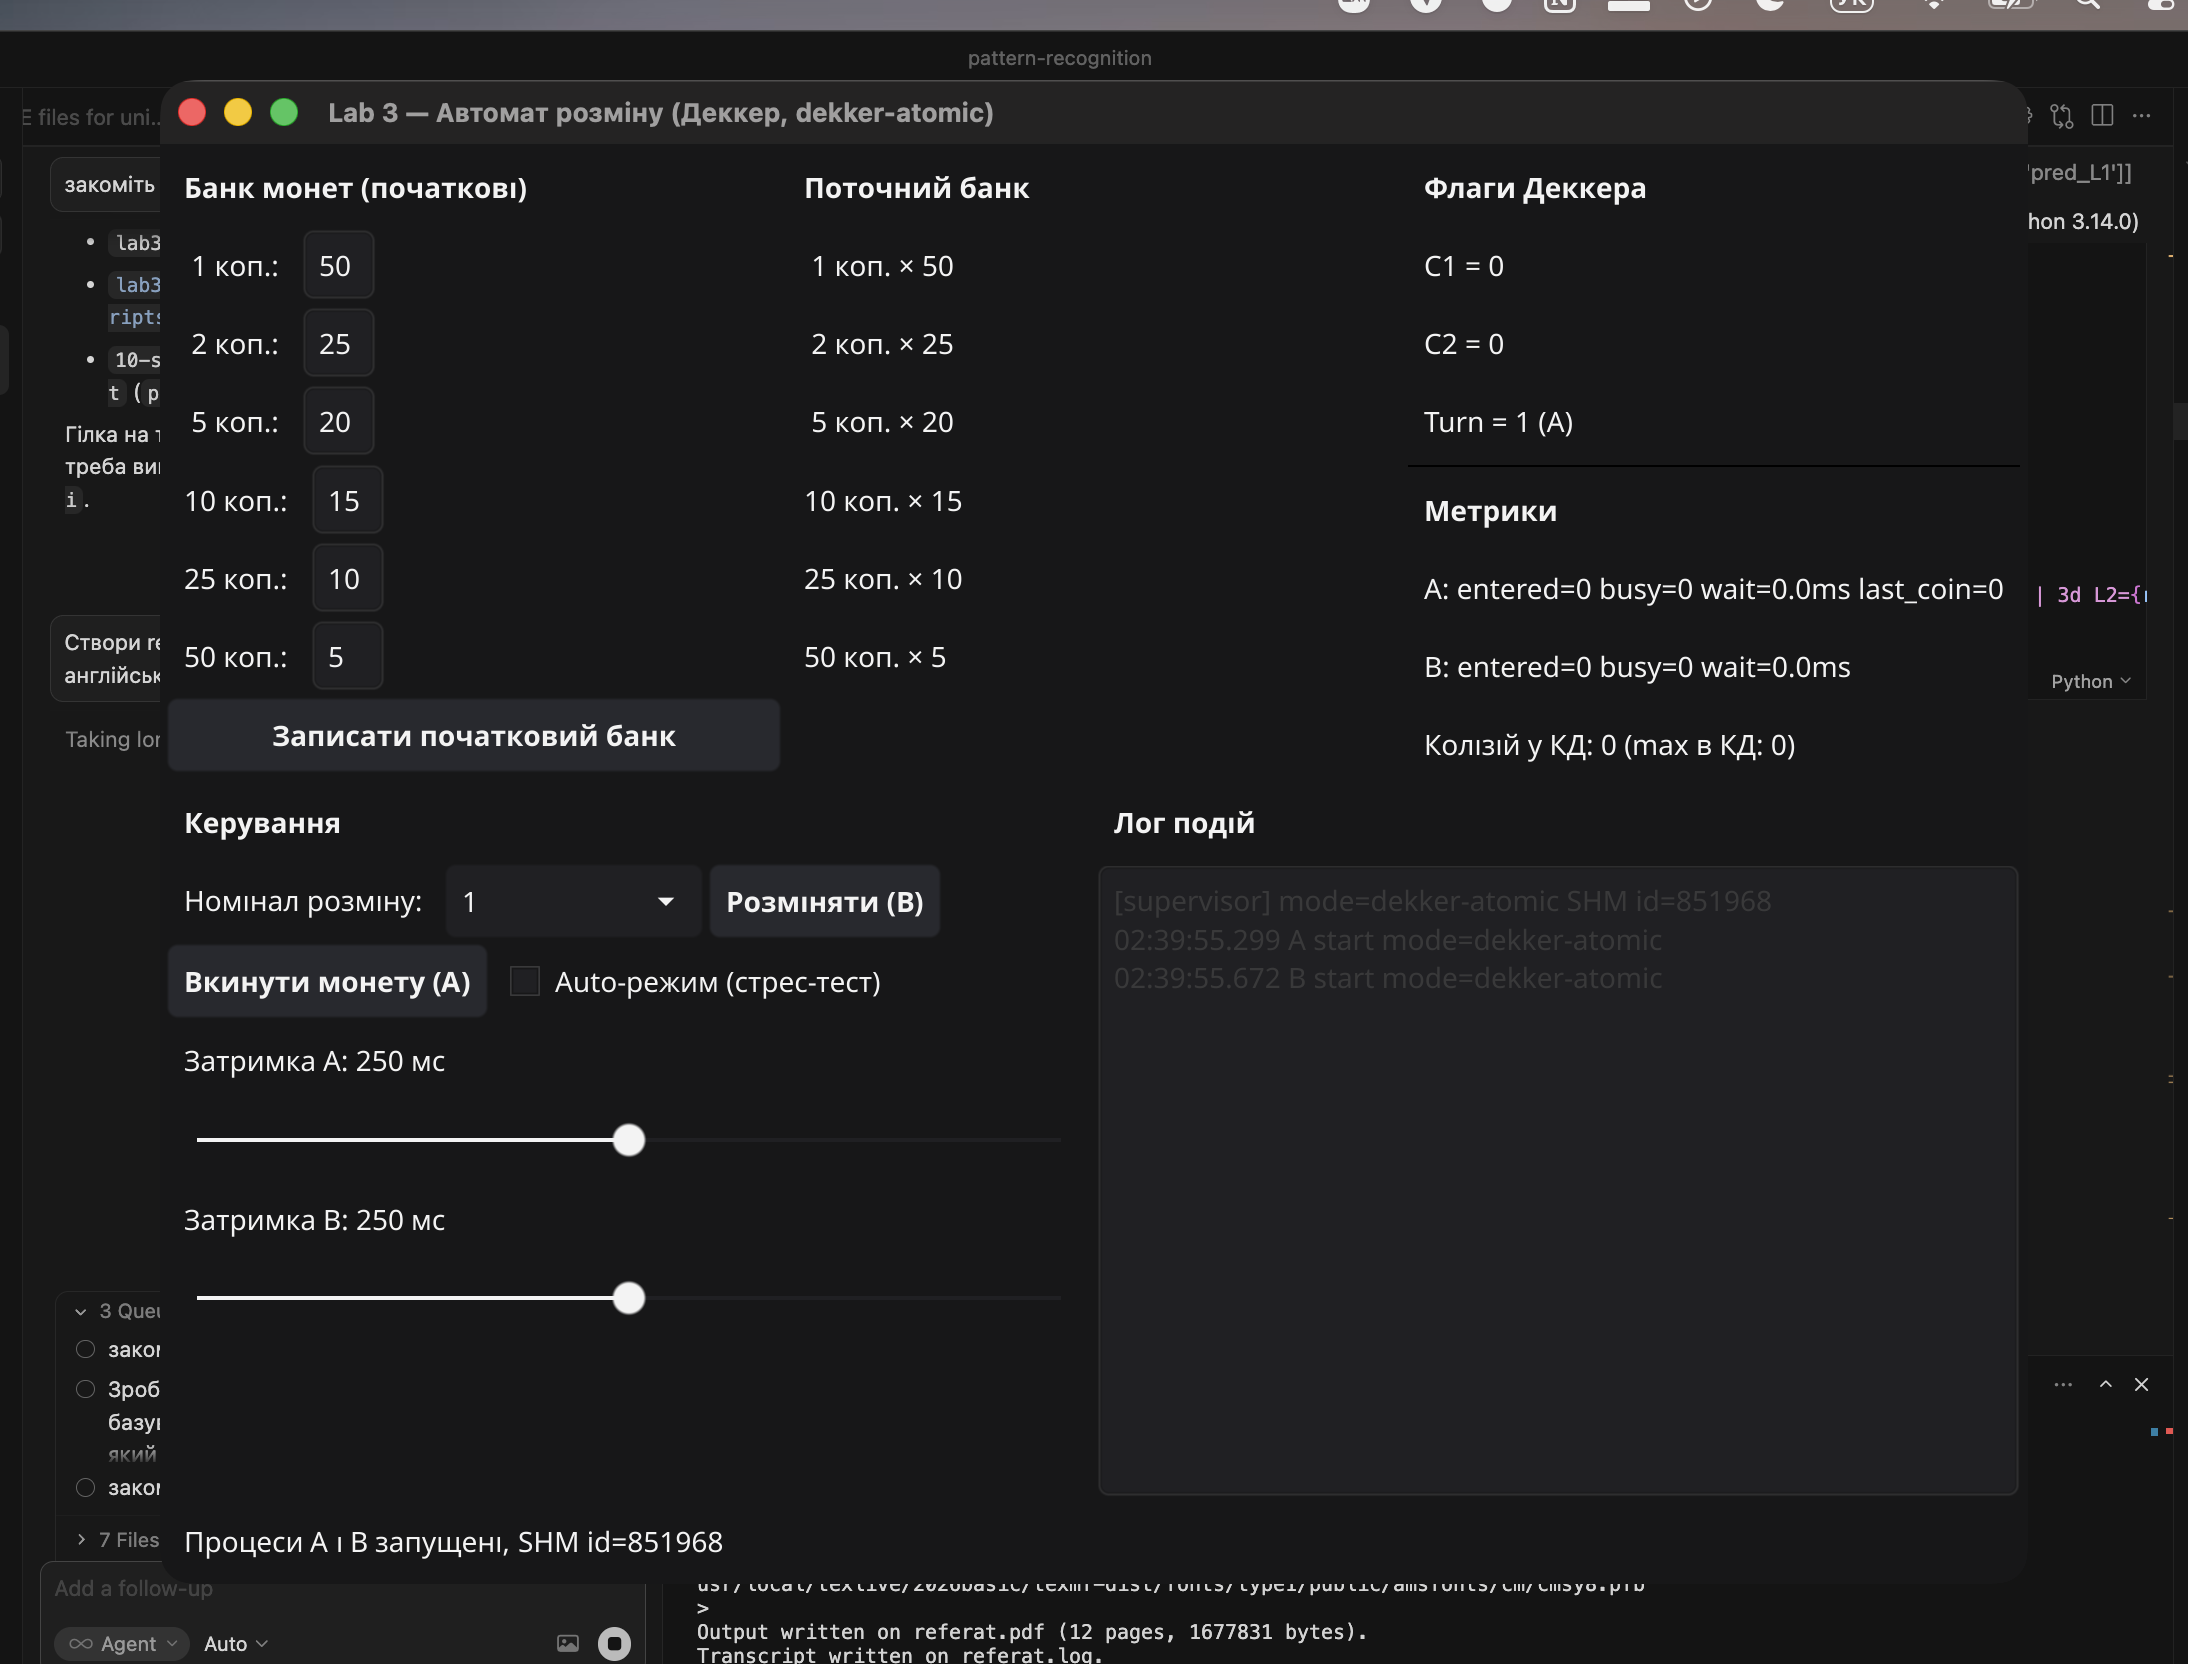
\includegraphics[width=\linewidth]{../screenshots/01-startup.png}
\caption{Стартовий стан супервізора після запуску. Банк =
50/25/20/15/10/5, прапорці Деккера в нулі, метрики порожні, у лозі лише
події \texttt{start} обох процесів.}
\end{figure}

\begin{figure}[H]
\centering
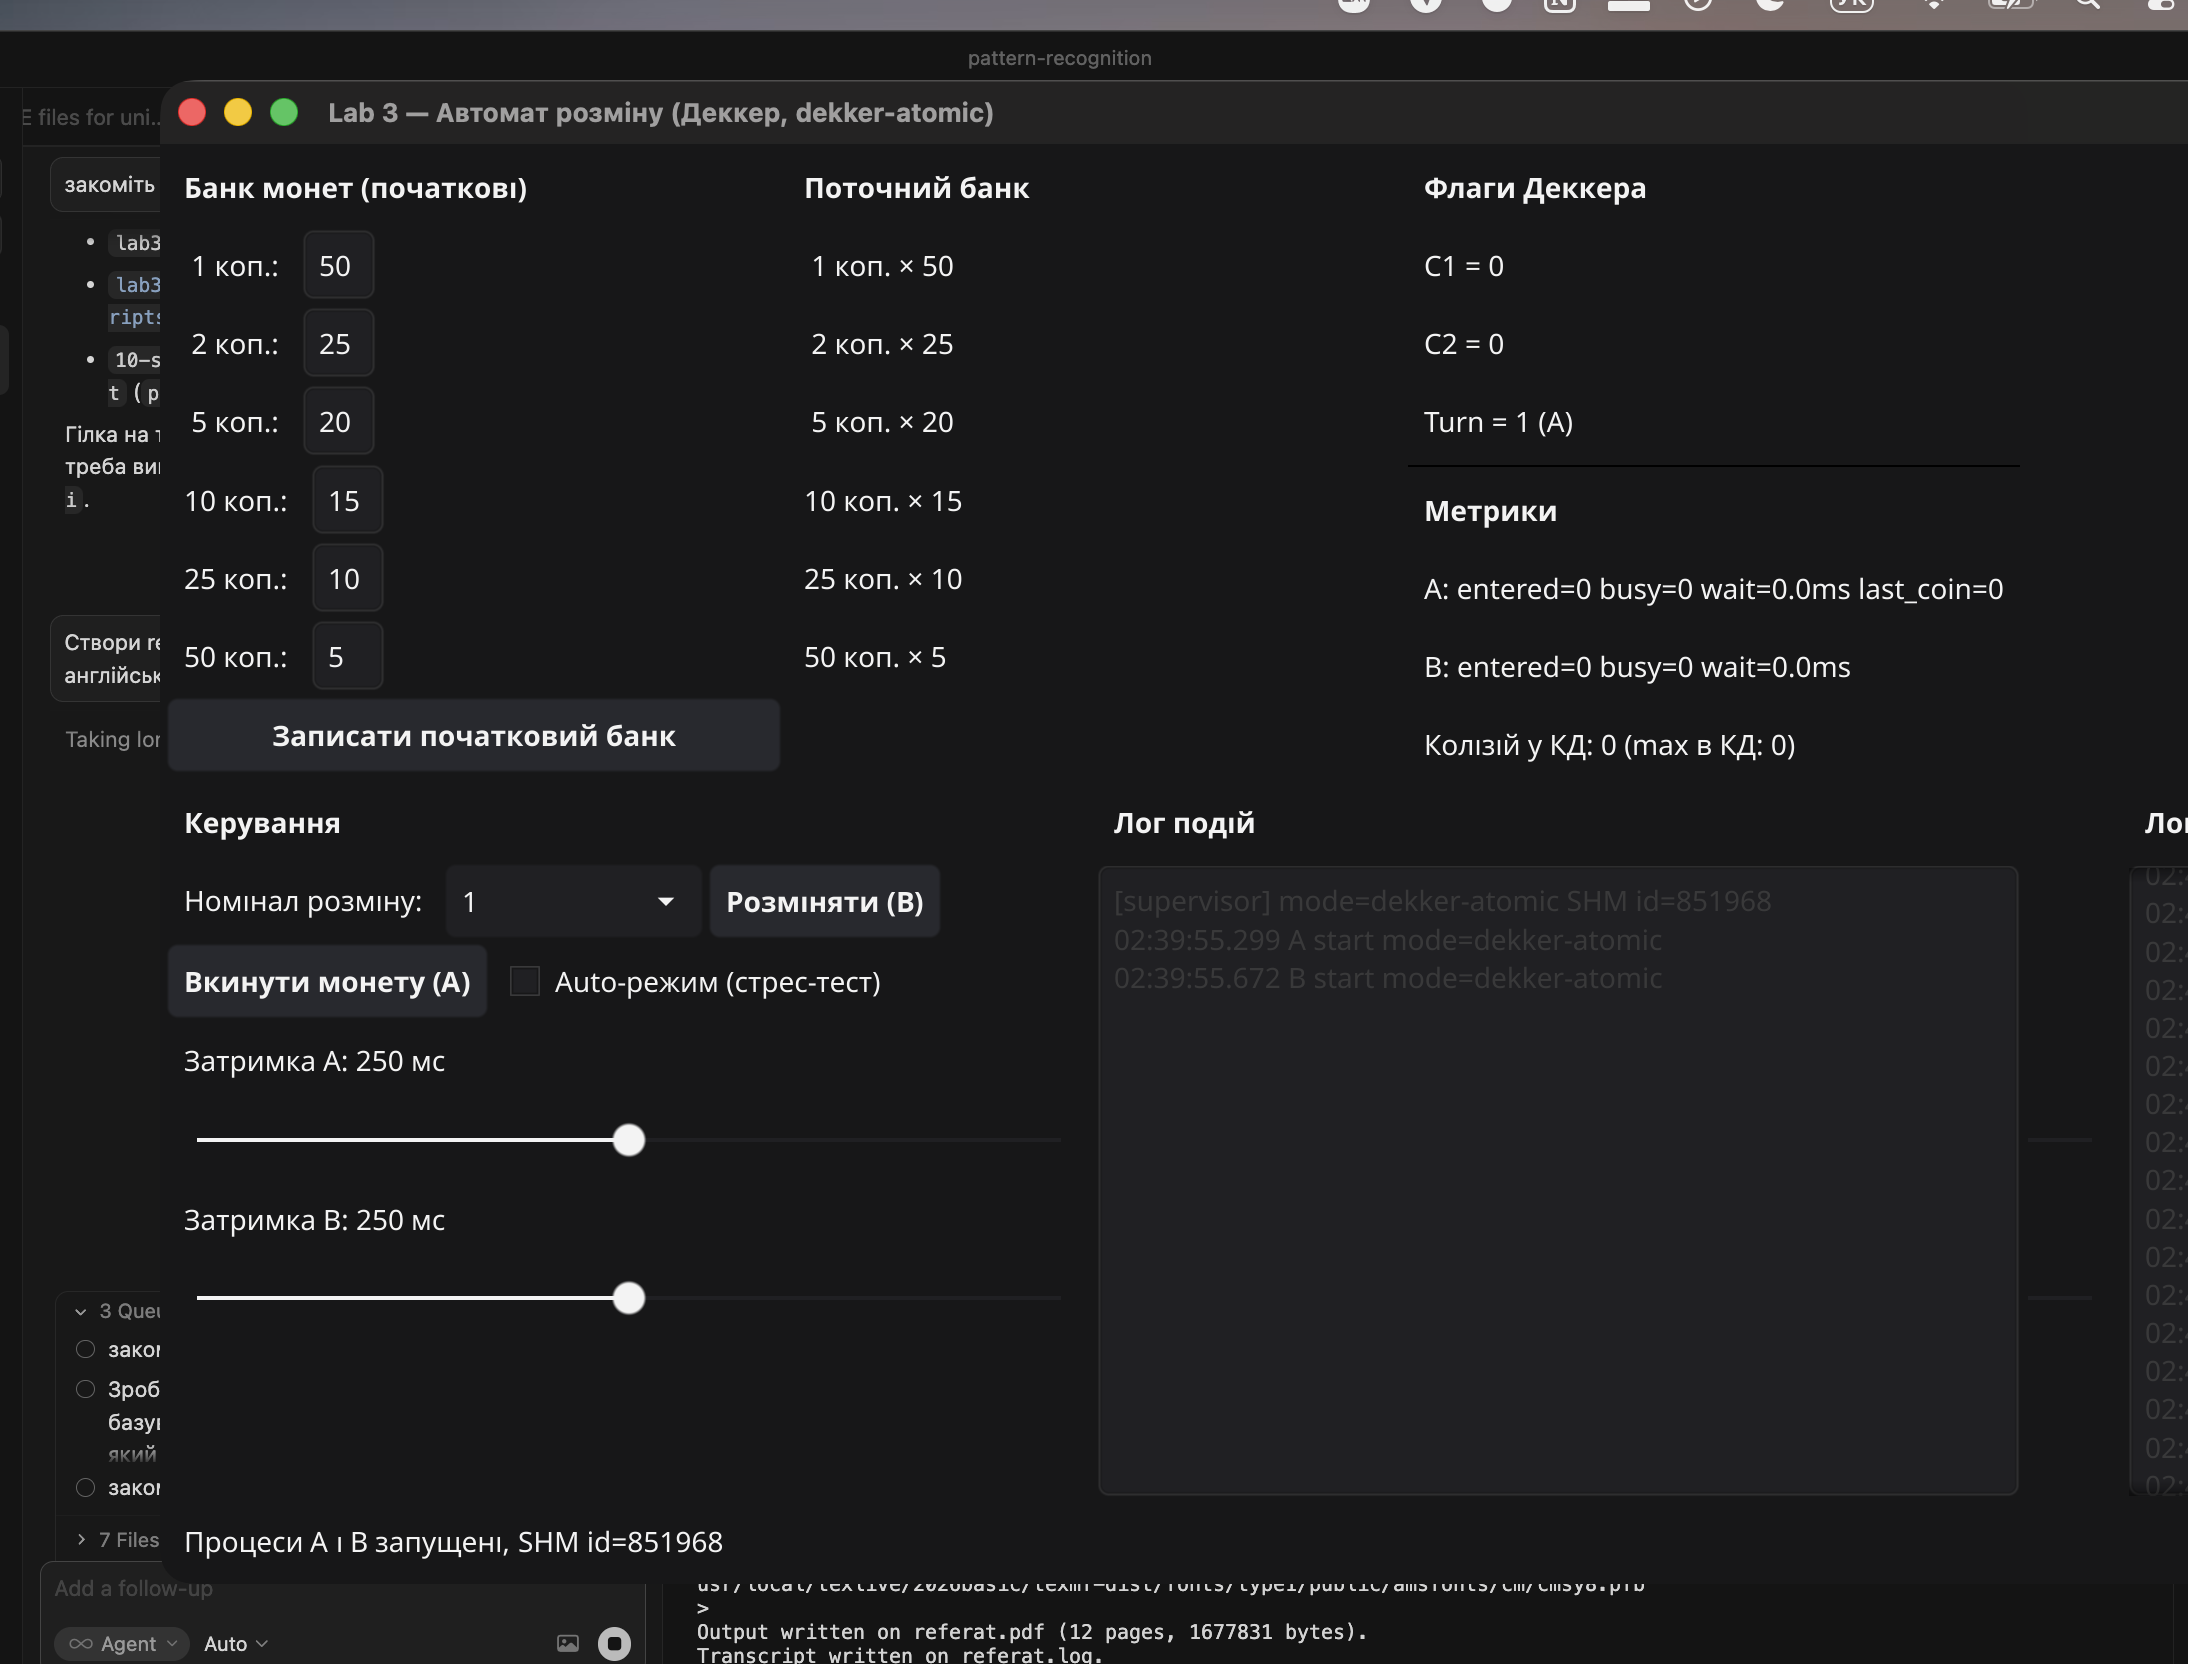
\includegraphics[width=\linewidth]{../screenshots/02-automode.png}
\caption{Робота автомата в auto-режимі \char`\~5\,с. Лічильники
$\text{EnterA} = \text{EnterB} \approx 23$, \textbf{Колізій у КД: 0},
max~в~КД: 1. У лозі видно правильне чергування
\texttt{enter\_cs}\,$\to$\,\texttt{deposit}\,$\to$\,\texttt{leave\_cs}
для~A і \texttt{enter\_cs}\,$\to$\,\texttt{deal}\,$\to$\,\texttt{leave\_cs}
для~B.}
\end{figure}

Метрики стрес-тесту (3~секунди):

\begin{lstlisting}[basicstyle=\ttfamily\footnotesize]
== Metrics after 3s (default-atomic) ==
  EnterA=516 EnterB=506
  BusyA=584  BusyB=63
  Wait msA=0.23 msB=0.12
  CS collisions=0 max-in-CS=1
\end{lstlisting}

\textbf{Висновок.} Atomic-варіант алгоритму Деккера забезпечує строге
взаємовиключення (\texttt{max-in-CS = 1}, колізії~=~0) і справедливий
розподіл часу між процесами ($\text{EnterA} \approx \text{EnterB}$).

\subsection{Ручне керування --- успішний розмін}

\begin{figure}[H]
\centering
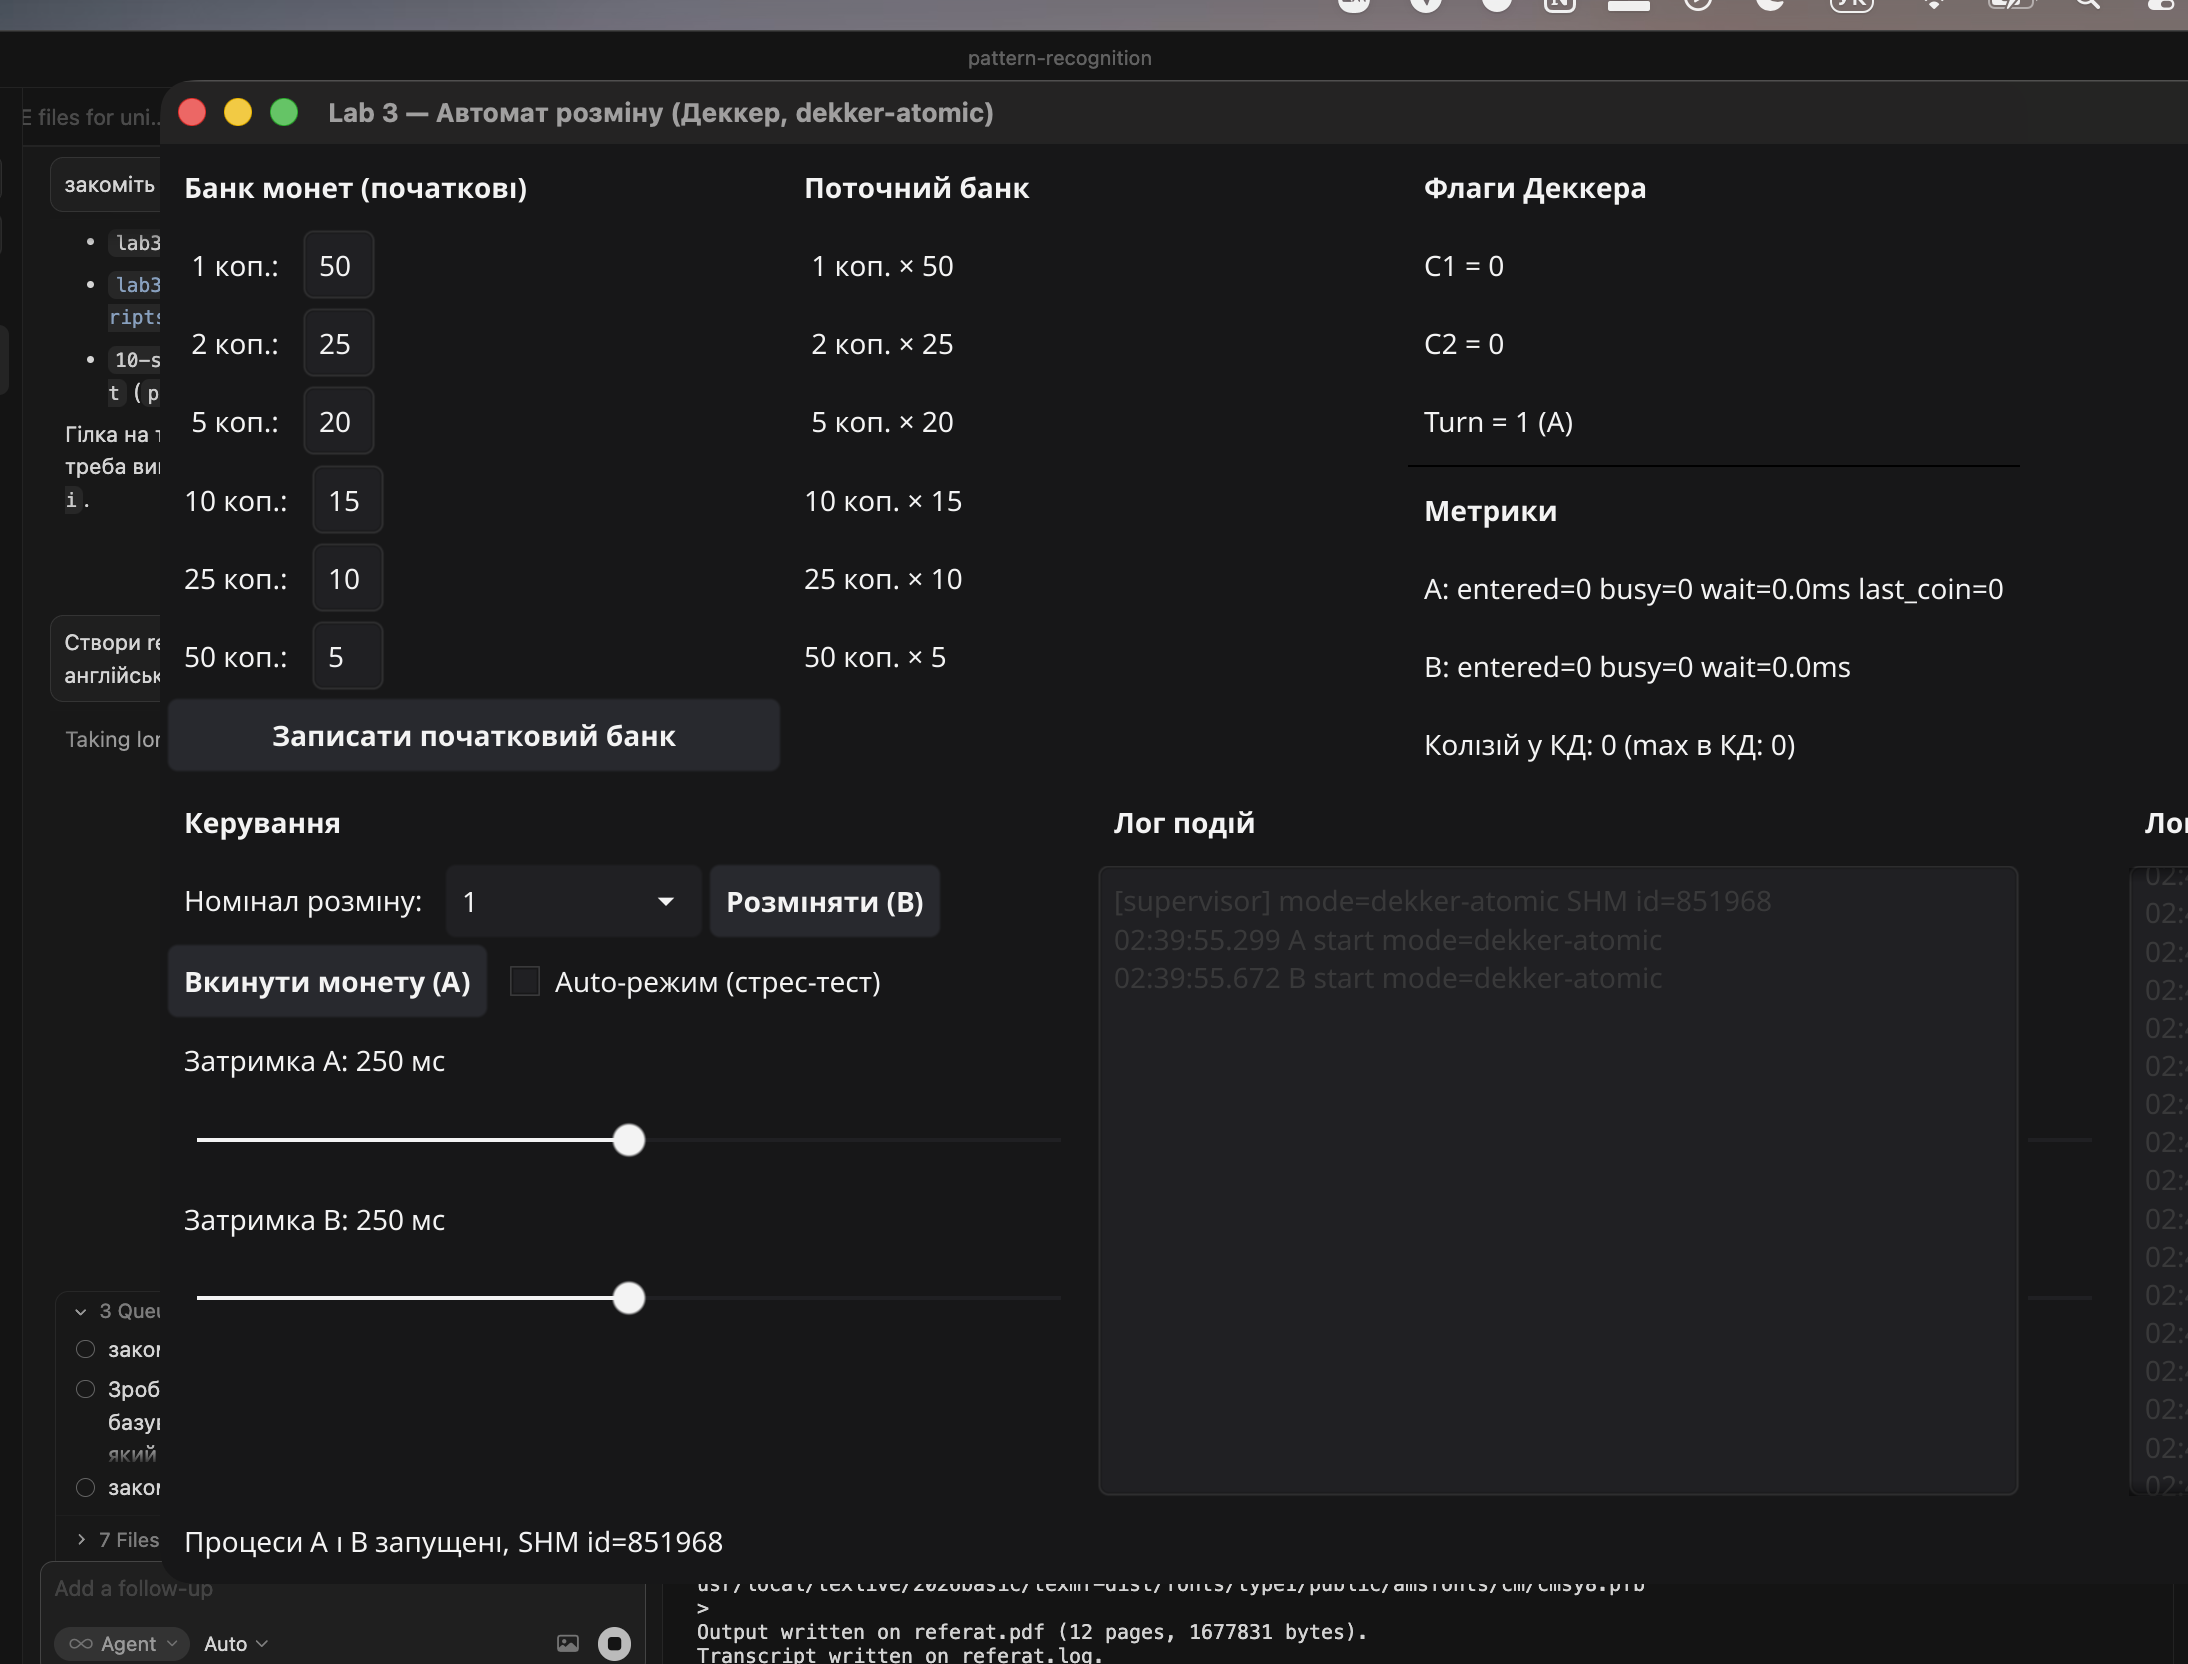
\includegraphics[width=\linewidth]{../screenshots/04-manual-deal.png}
\caption{Сценарій з кнопками: процес~A прийняв монети, процес~B
розміняв їх. Лог показує цикли
\texttt{enter\_cs}\,$\to$\,\texttt{deal}\,$\to$\,\texttt{leave\_cs}
без колізій.}
\end{figure}

\subsection{Ручне керування --- відмова}

\begin{figure}[H]
\centering
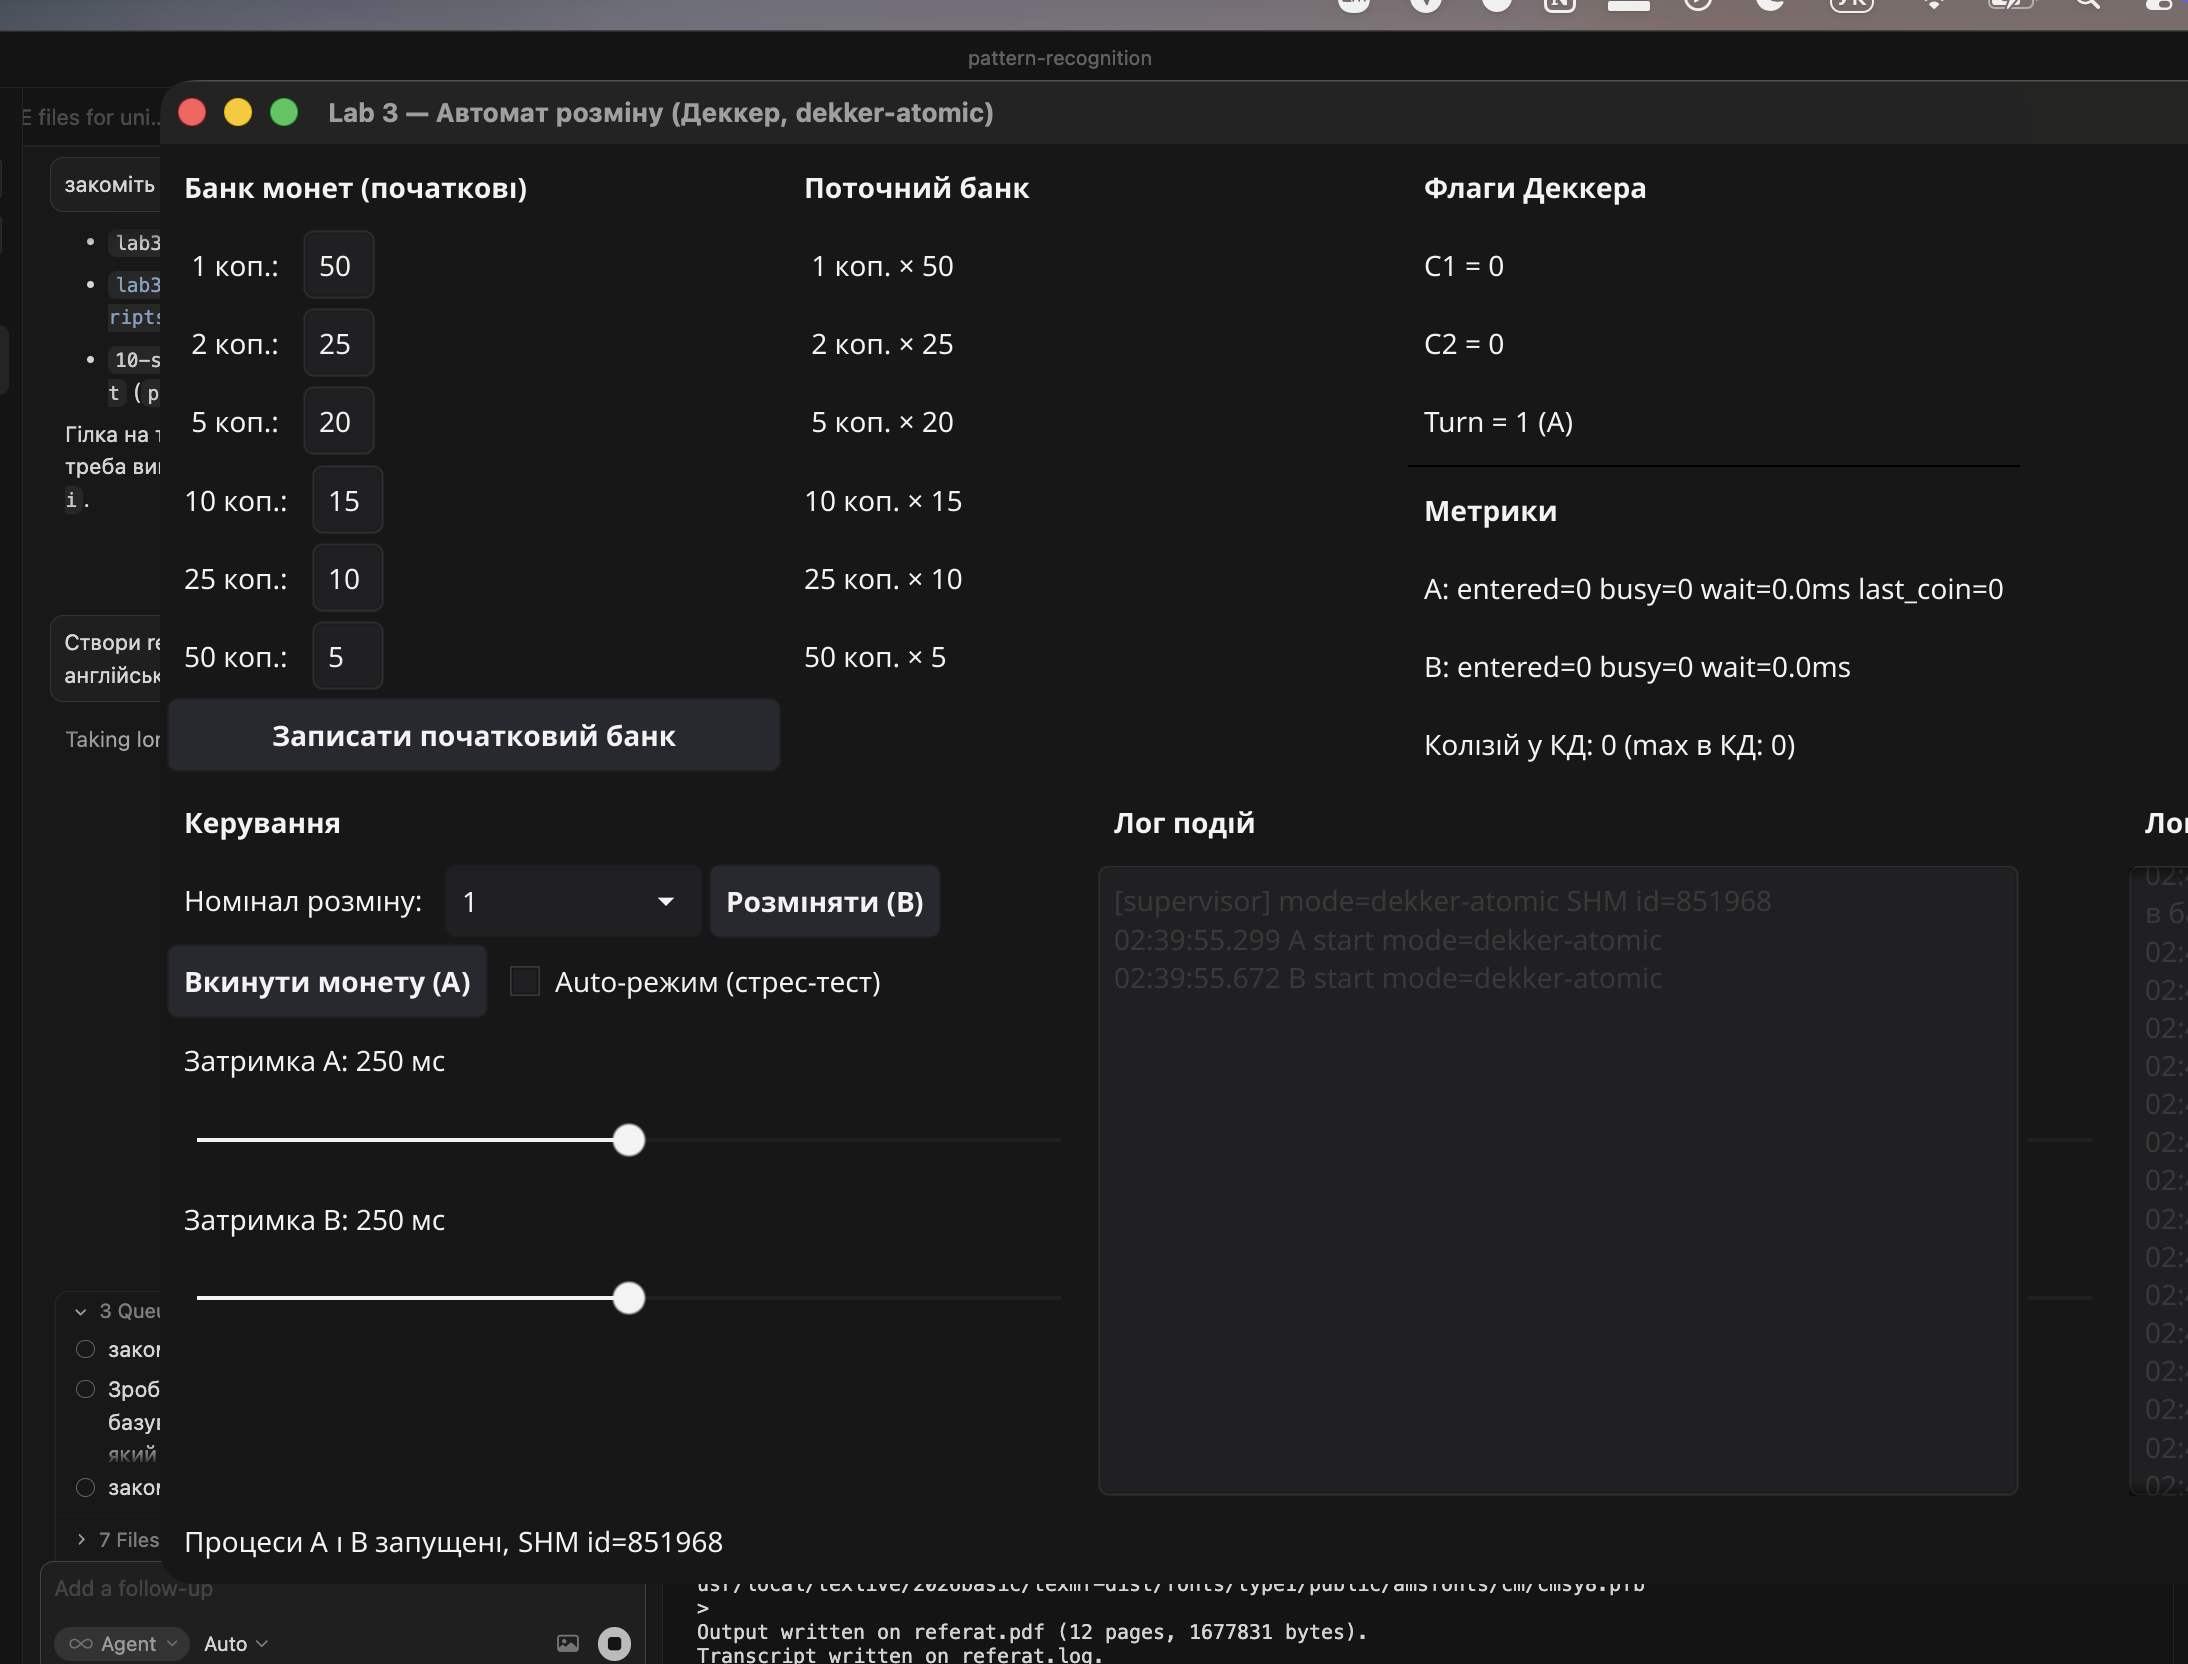
\includegraphics[width=\linewidth]{../screenshots/05-manual-refuse.png}
\caption{Запит <<розміняти 2~коп. на 50~коп.>> --- процес~B повертає
\texttt{refuse=2} <<номінал розміну не менший за монету>>. У лозі видно
серію таких відмов з різними коп. на 50.}
\end{figure}

\subsection{Без синхронізації --- порушення взаємовиключення}

\begin{figure}[H]
\centering
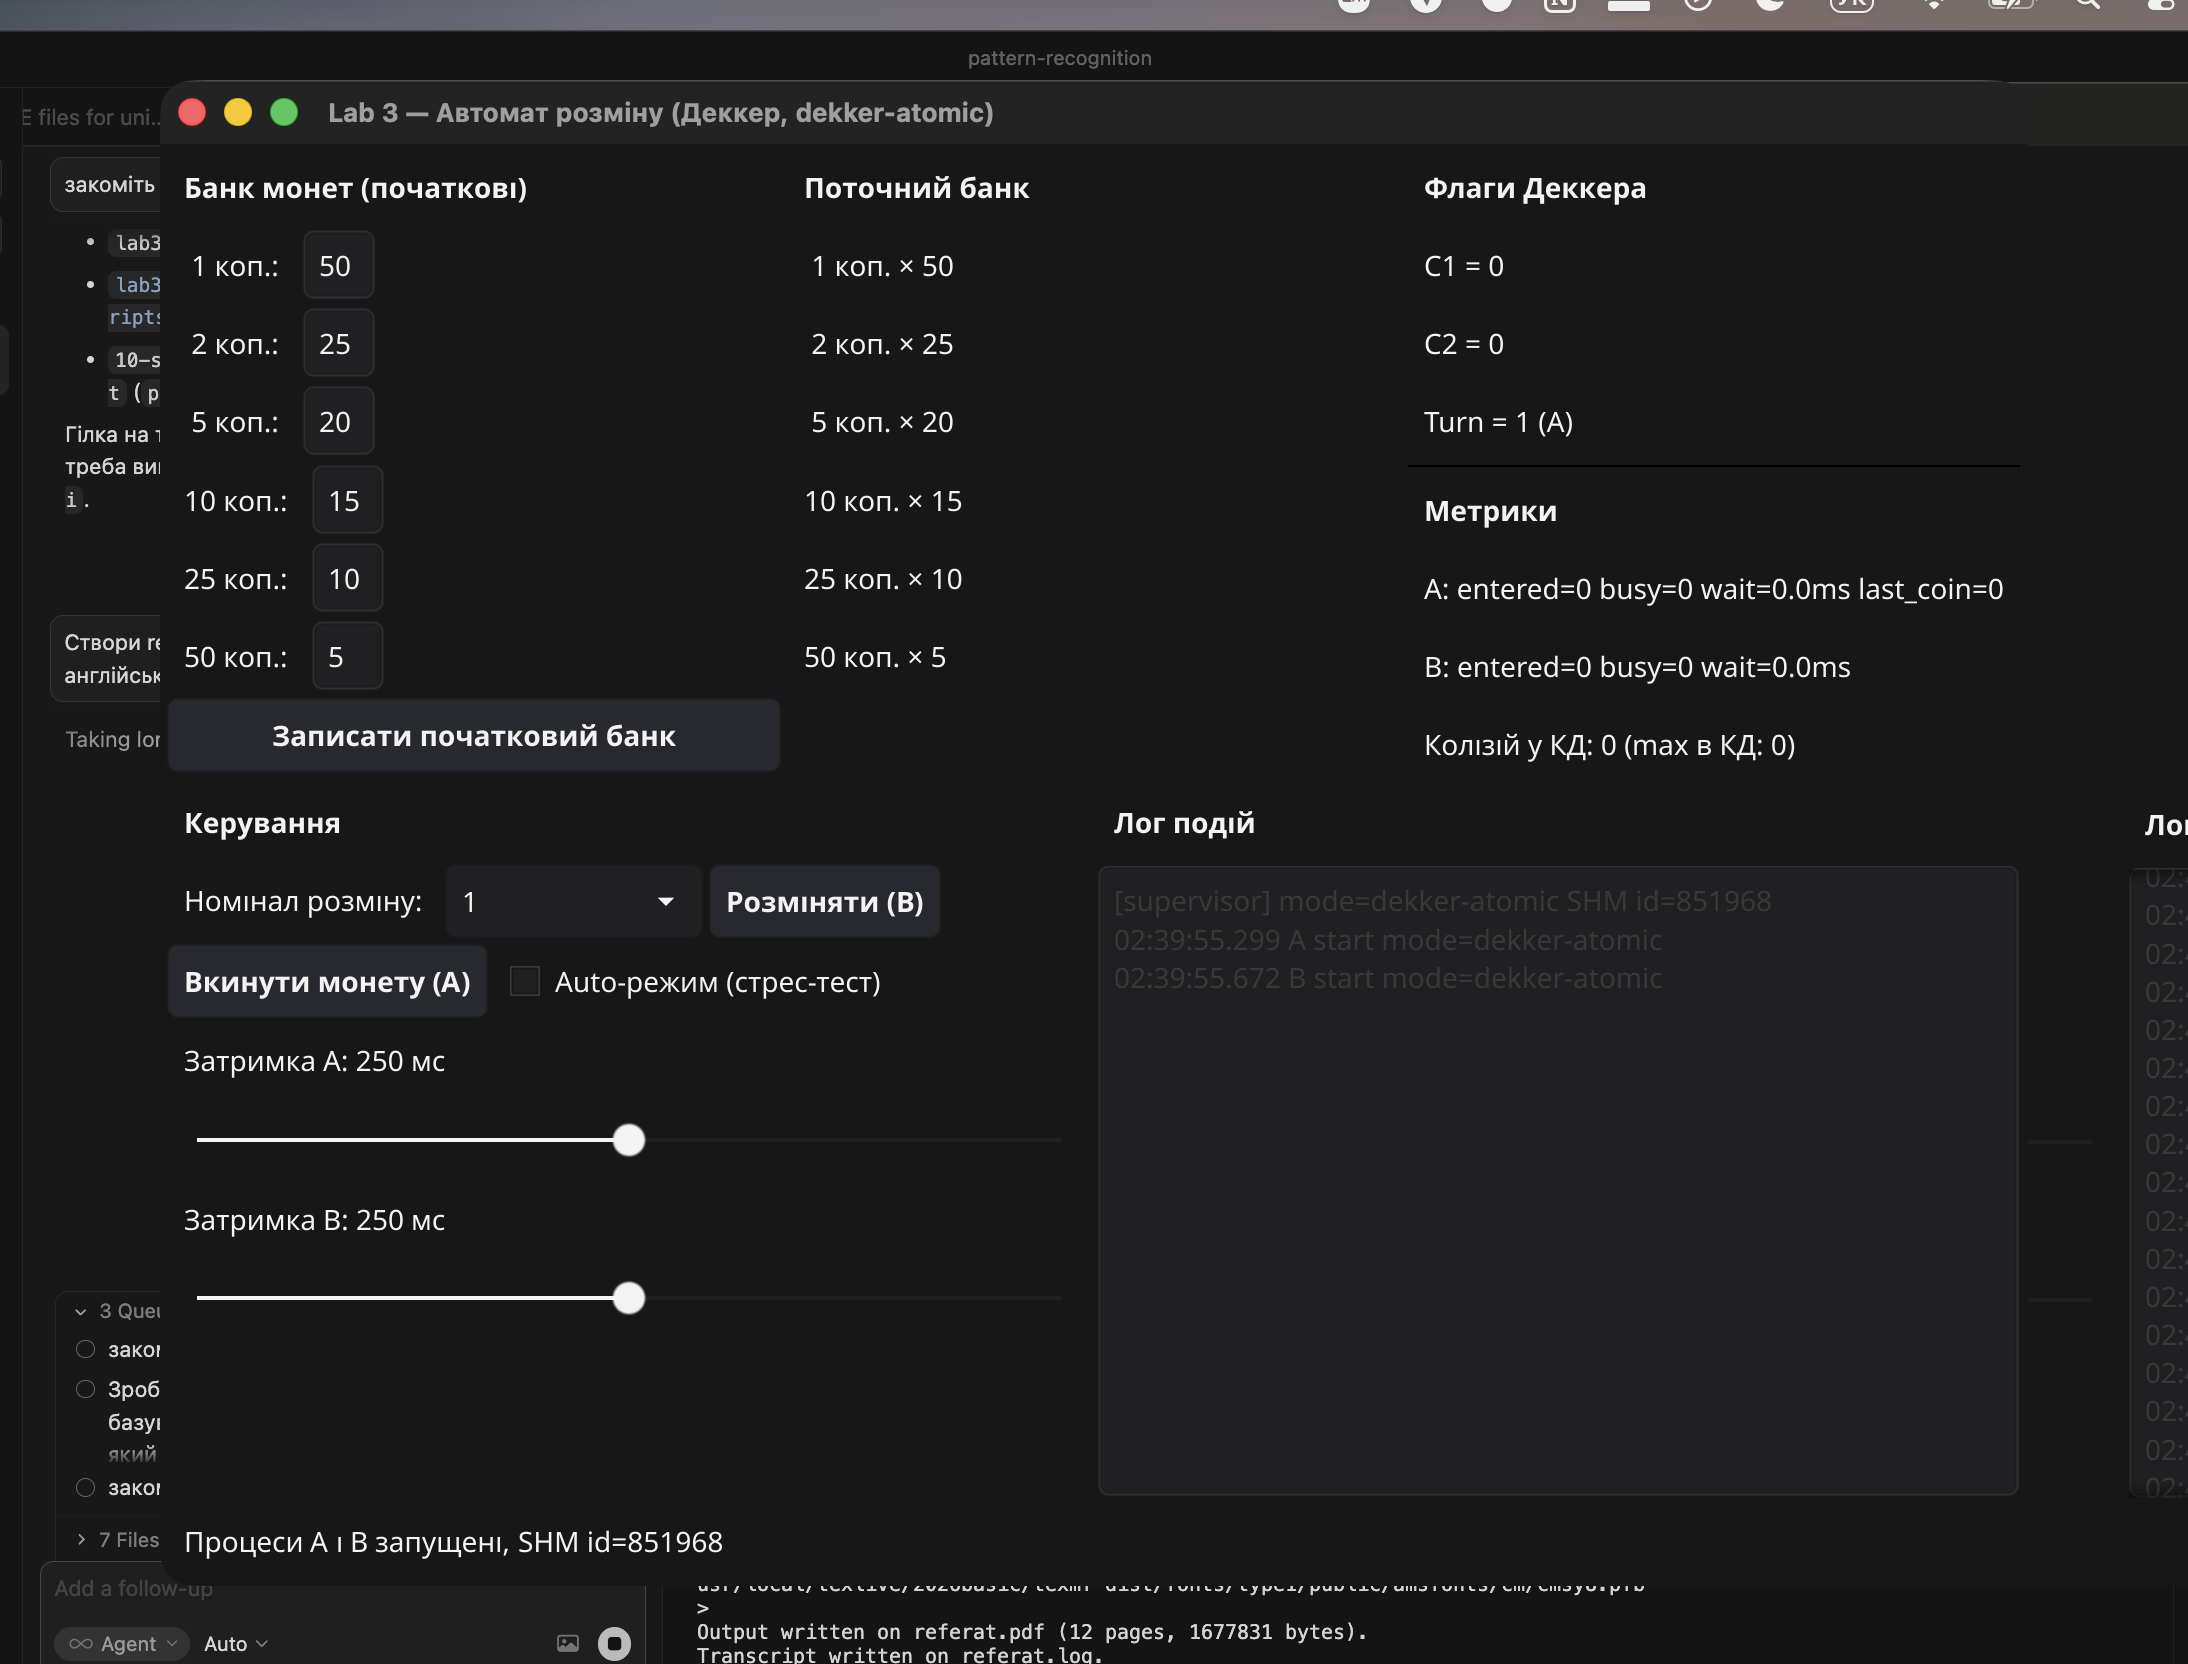
\includegraphics[width=\linewidth]{../screenshots/03-nosync-collisions.png}
\caption{Той самий код, але \texttt{Enter}/\texttt{Leave} Деккера
підмінені на no-op (\texttt{build -tags=nosync}). Уже після 5~секунд
auto-mode лічильник <<Колізій у КД>> дорівнює \textbf{19},
max~в~КД~=~2 --- експериментальне підтвердження одночасного перебування
A і B у КД.}
\end{figure}

Метрики стрес-тесту:

\begin{lstlisting}[basicstyle=\ttfamily\footnotesize]
== Metrics after 3s (nosync) ==
  EnterA=505 EnterB=467
  BusyA=0  BusyB=0
  Wait msA=0.00 msB=0.00
  CS collisions=18 max-in-CS=2
\end{lstlisting}

\textbf{Висновок.} Без жодної синхронізації обидва процеси входять у~КД
одночасно \char`\~18 разів за 3 секунди (\char`\~6~разів на секунду),
і це негайно проявляється у непослідовних значеннях банку (наприклад,
B може видавати решту з банку, який~A ще не встиг оновити).

\subsection{Racy-варіант (без sync/atomic)}

\begin{lstlisting}[basicstyle=\ttfamily\footnotesize]
== Metrics after 3s (racy) ==
  EnterA=489 EnterB=410
  BusyA=983  BusyB=664
  Wait msA=0.36 msB=0.29
  CS collisions=0 max-in-CS=1
\end{lstlisting}

На macOS arm64 у нашій конфігурації racy-варіант \textbf{не зловив
колізію за 3~с}. Це не означає, що алгоритм коректний --- це означає,
що вікно реордерингу між непослідовним записом \texttt{C[self]:=1} і
читанням \texttt{C[other]} дуже вузьке (одиниці--десятки наносекунд),
а між двома КД ще є виклик \texttt{runtime.Gosched()} плюс
\texttt{time.Sleep}, які діють як часткові бар'єри. Для лабораторної
достатньо того, що:
\begin{itemize}
    \item В умові Деккера явно припускається <<блокування пам'яті>>
    (с.\,5), тобто послідовна консистентність --- це фактично і є те,
    що дає \texttt{atomic}.
    \item Варіант \texttt{nosync} (рис.~5) демонструє, що
    <<живий>> race condition виникає миттєво, коли немає
    взаємовиключення взагалі.
\end{itemize}

\subsection{Влив затримок на справедливість}

При зменшенні \texttt{DelayMsA} до 0 і збільшенні \texttt{DelayMsB} до
300~мс лічильник \texttt{BusyA} стрімко зростає (A крутиться у
внутрішньому циклі \texttt{while Turn == other}), а $\text{EnterA}
\approx \text{EnterB}$ --- Деккерова змінна \texttt{Turn} не дає A
відірватися. Це чисте підтвердження властивості bounded waiting для
двох процесів.

% ============================================================
\section{Висновки}
% ============================================================

\begin{enumerate}
    \item \textbf{Класичний алгоритм Деккера успішно розв'язує задачу
    взаємовиключення двох процесів} з лише поділюваною пам'яттю --- у
    нашому експерименті це підтверджено нульовими колізіями за 3
    секунди інтенсивної роботи ($\text{EnterA} = 516$, $\text{EnterB} =
    506$).

    \item \textbf{Активне очікування --- головний недолік}: у
    atomic-режимі сумарно накопичено \char`\~600 ітерацій busy-wait на
    A і \char`\~60 на B. Це гірше, ніж у семафорах, де процес
    блокується операційною системою.

    \item \textbf{Алгоритм не масштабується тривіально на $N>2$
    процесів} --- для більше двох процесів структури \texttt{C1},
    \texttt{C2}, \texttt{Turn} потрібно узагальнювати (наприклад,
    алгоритм Бейкері Лампорта).

    \item \textbf{На сучасних CPU потрібні memory barrier'и.} Без них
    (у нашому \texttt{racy}-режимі) алгоритм формально некоректний,
    хоча короткотривалі тести можуть випадково <<проскочити>> завдяки
    \texttt{runtime.Gosched}. Стандартний спосіб лікування --- атомарні
    операції з seq-cst (як у нашій основній реалізації).

    \item \textbf{Real-process model + System V SHM} --- повноцінна
    модель для курсу ОС. На відміну від рішення goroutine'ами, тут
    видно справжній IPC: \texttt{shmget}/\texttt{shmat}/\texttt{shmctl(IPC\_RMID)},
    передача дескриптора через \texttt{ENV}, лайфсайкл сегмента під
    керуванням батьківського процесу, ризик <<осиротілих>> сегментів
    за неакуратного завершення (вирішується через \texttt{ipcs -m} +
    \texttt{ipcrm}, або \texttt{make clean}).

    \item \textbf{Порівняно з іншими засобами синхронізації} (семафори
    --- варіант~1, поштові скриньки --- варіант~3, Test\&Set ---
    варіант~4):
    \begin{itemize}
        \item Деккер виграє у переносимості: не потребує апаратних
        команд або системних викликів.
        \item Програє у простоті: код для двох процесів уже досить
        обширний, а псевдокод з підручника для $N$ процесів буде дуже
        громіздким.
        \item Програє у CPU-efficiency: семафор з блокуванням у ядрі
        не палить процесор.
    \end{itemize}
\end{enumerate}

% ============================================================
\section{Як відтворити результати}
% ============================================================

\begin{lstlisting}[basicstyle=\ttfamily\footnotesize]
cd lab3
make tidy            # пiдтягнути Fyne v2
make build           # зiбрати bin/supervisor, bin/process_a, bin/process_b
make run             # запустити GUI

# Стрес-тест (метрики у трьох режимах):
DURATION=3s ./examples/stress.sh

# Швидко перемкнути auto-режим/затримки без GUI:
./bin/poke --auto on
./bin/poke --delay-a 0 --delay-b 200
./bin/poke --print
\end{lstlisting}

% ============================================================
\section{Перелік файлів}
% ============================================================

\begin{table}[H]
\footnotesize
\begin{tabularx}{\linewidth}{@{}l L@{}}
\toprule
\textbf{Файл} & \textbf{Опис} \\
\midrule
\texttt{cmd/supervisor/main.go}             & Fyne GUI + життєвий цикл SHM + спавн процесів \\
\texttt{cmd/process\_a/main.go}             & Процес A: прийом монети, вхід у КД, mailbox \\
\texttt{cmd/process\_b/main.go}             & Процес B: розмін, оновлення банку \\
\texttt{internal/shm/shm\_sysv.go}          & cgo-обгортка \texttt{shmget}/\texttt{shmat}/\texttt{shmdt}/\texttt{shmctl} \\
\texttt{internal/shm/state.go}              & Layout спільного \texttt{struct State} \\
\texttt{internal/dekker/dekker\_default.go} & Канонічний Деккер з \texttt{sync/atomic} \\
\texttt{internal/dekker/dekker\_racy.go}    & Demo: Деккер без atomic (\texttt{racy}) \\
\texttt{internal/dekker/dekker\_nosync.go}  & Demo: no-op Enter/Leave (\texttt{nosync}) \\
\texttt{internal/coinbank/bank.go}          & \texttt{MakeChange}, 4 коди відмов \\
\texttt{internal/coinbank/bank\_test.go}    & Юніт-тести 8 сценаріїв \\
\texttt{internal/ipc/events.go}             & JSON-протокол подій \\
\texttt{examples/smoketest/main.go}         & Headless run + друк метрик \\
\texttt{examples/poke/main.go}              & CLI-помічник: тоглити прапорці SHM \\
\texttt{examples/stress.sh}                 & Послідовний прогін трьох build-tags \\
\texttt{screenshots/}                       & Скріни GUI для звіту \\
\bottomrule
\end{tabularx}
\end{table}

\end{document}
